\documentclass[aps,prl,twocolumn,groupedaddress]{revtex4-1}
% \documentclass[aps,twocolumn,secnumarabic,balancelastpage,amsmath,amssymb,nofootinbib]{revtex4-1}
\usepackage{amsmath}
\usepackage{amssymb}
\usepackage{amsfonts}
\usepackage{color}
\usepackage{graphics}
\usepackage[pdftex]{graphicx}
\usepackage[utf8x]{inputenc}
\usepackage[colorlinks=true]{hyperref}

\newcommand{\ud}{\mathrm{d}}
\newcommand{\ue}{\mathrm{e}}
\newcommand{\ui}{\mathrm{i}}
\newcommand{\res}{\mathrm{Res}}
\newcommand{\Tr}{\mathrm{Tr}}
\newcommand{\dsum}{\displaystyle\sum}
\newcommand{\dprod}{\displaystyle\prod}
\newcommand{\dlim}{\displaystyle\lim}
\newcommand{\dint}{\displaystyle\int}
\newcommand{\fsno}[1]{{\!\not\!{#1}}}
\newcommand{\texp}[2]{\ensuremath{{#1}\times10^{#2}}}
\newcommand{\dexp}[2]{\ensuremath{{#1}\cdot10^{#2}}}
\newcommand{\eval}[2]{{\left.{#1}\right|_{#2}}}
\newcommand{\paren}[1]{{\left({#1}\right)}}
\newcommand{\lparen}[1]{{\left({#1}\right.}}
\newcommand{\rparen}[1]{{\left.{#1}\right)}}
\newcommand{\abs}[1]{{\left|{#1}\right|}}
\newcommand{\sqr}[1]{{\left[{#1}\right]}}
\newcommand{\crly}[1]{{\left\{{#1}\right\}}}
\newcommand{\angl}[1]{{\left\langle{#1}\right\rangle}}
\newcommand{\tpdiff}[4][{}]{{\paren{\frac{\partial^{#1} {#2}}{\partial {#3}{}^{#1}}}_{#4}}}
\newcommand{\tpsdiff}[4][{}]{{\paren{\frac{\partial^{#1}}{\partial {#3}{}^{#1}}{#2}}_{#4}}}
\newcommand{\pdiff}[3][{}]{{\frac{\partial^{#1} {#2}}{\partial {#3}{}^{#1}}}}
\newcommand{\diff}[3][{}]{{\frac{\ud^{#1} {#2}}{\ud {#3}{}^{#1}}}}
\newcommand{\psdiff}[3][{}]{{\frac{\partial^{#1}}{\partial {#3}{}^{#1}} {#2}}}
\newcommand{\sdiff}[3][{}]{{\frac{\ud^{#1}}{\ud {#3}{}^{#1}} {#2}}}
\newcommand{\tpddiff}[4][{}]{{\left(\dfrac{\partial^{#1} {#2}}{\partial {#3}{}^{#1}}\right)_{#4}}}
\newcommand{\tpsddiff}[4][{}]{{\paren{\dfrac{\partial^{#1}}{\partial {#3}{}^{#1}}{#2}}_{#4}}}
\newcommand{\pddiff}[3][{}]{{\dfrac{\partial^{#1} {#2}}{\partial {#3}{}^{#1}}}}
\newcommand{\ddiff}[3][{}]{{\dfrac{\ud^{#1} {#2}}{\ud {#3}{}^{#1}}}}
\newcommand{\psddiff}[3][{}]{{\frac{\partial^{#1}}{\partial{}^{#1} {#3}} {#2}}}
\newcommand{\sddiff}[3][{}]{{\frac{\ud^{#1}}{\ud {#3}{}^{#1}} {#2}}}
\newcommand{\eff}{ef\! f}
\newcommand{\fxnote}[1]{{\textbf{[#1]}}}

\begin{document}
\title{Motional Ground State Cooling Outside the Lamb-Dicke Regime}
\author{Y. Yu}
\email{yichaoyu@g.harvard.edu}
\author{N. R. Hutzler}
\altaffiliation{Present address: California Institute of Technology, Division of Physics, Mathematics, and Astronomy. Pasadena, CA, 91125}
\author{J. T. Zhang}
\author{L. R. Liu}
\author{T. Rosenband}
\author{K.-K. Ni}
\email{ni@chemistry.harvard.edu}
\affiliation{Department of Chemistry and Chemical Biology, Harvard University, Cambridge, Massachusetts, 02138, USA}
\affiliation{Department of Physics, Harvard University, Cambridge, Massachusetts, 02138, USA}
\affiliation{Harvard-MIT Center for Ultracold Atoms, Cambridge, Massachusetts, 02138, USA}

\date{\today}

\begin{abstract}
  We report Raman sideband cooling of a single sodium atom to its three-dimensional
  motional ground state in an optical tweezer.
  Despite a large Lamb-Dicke parameter, high initial temperature, and
  large differential light shifts between the excited state and the ground state,
  we achieve a ground state population of $81(4)$\% after $100$ ms of cooling, for the 85\% of atoms that survive cooling and re-imaging.
  Our technique includes addressing high-order sidebands, where several motional quanta are removed by a single laser pulse, and
  fast modulation of the optical tweezer intensity.
  We demonstrate that Raman sideband cooling to the 3D motional ground state is possible, even without tight confinement and low initial temperature.
  % This is particularly relevant for systems which are challenging to laser-cool, such as molecules and exotic atoms, and opens up the possibility to gain quantum motional control of these systems.
\end{abstract}

\maketitle


% Systems of trapped neutral atoms assembled from the bottom-up in an array of optical tweezers are a promising platform to study quantum information and quantum simulations~
Trapped neutral atoms, assembled in an array of optical tweezers, are a promising platform to study quantum information and quantum simulations~
\cite{Schlosser2001,Weiss2004,Isenhower2010,Wilk2010,Kaufman2015,Labuhn2016,Murmann2015}.
The inherent single-particle detection and control, combined with tunable interactions,
allow implementations of neutral-atom-based quantum logic gates~\cite{Isenhower2010,Wilk2010},
novel quantum phases~\cite{Labuhn2016}, and single-photon switches~\cite{Dayan2008,Tiecke2014}.
Advances in real-time re-arrangement of optical tweezers enable rapid preparation of atoms
in large and complex geometries~\cite{Barredo2016,Endres2016}.
Quantum motional control of individual
atoms~\cite{Li2012,Kaufman2012,Thompson2013,Liu2017,Robens2017} enable
studies of the atomic Hong-Ou-Mandel effect~\cite{Kaufman2014},
high-fidelity single qubit gates~\cite{Wang2016},
and efficient coupling of single atoms to photonic crystal cavities~\cite{Thompson2013a}.

Extending optical tweezer arrays to include polar molecules will open a range of
new applications that exploit long-lived molecular internal states
and tunable long range interactions~\cite{DeMille2002,Gorshkov2011,Yan2013}.
Molecules could be assembled from atom pairs in optical tweezers~\cite{Liu2017},
or directly loaded from magneto-optical traps
(MOTs)~\cite{Barry2014,Truppe2017SubDoppler,Anderegg2017}.
For either approach, preparing the constituent atoms or molecules in the lowest motional
quantum state is important to realize long coherence times in quantum applications.

Preparation of single atoms in the motional ground state has been achieved in optical tweezers~\cite{Kaufman2012,Thompson2013,Liu2017,Robens2017}
 using Raman sideband cooling (RSC)~\cite{Monroe1995,Kerman2000,Han2000}.
However, RSC in these systems takes place in the Lamb-Dicke (LD) regime, where
the spread of the initial wavefunctions is smaller than the reduced wavelength of light ($\lambdabar$)
used to address them.
Systems with a large position spread ($z_{rms}$), either due to small mass or high initial temperature,
fall outside of the LD regime and undergo strong recoil heating during RSC.
In this letter we demonstrate cooling of single sodium atoms in optical tweezers,
initially outside the LD regime ($z_{rms}/\lambdabar=4.0$), to the motional ground state.
We achieve a 3D ground state population of $P_0=81(4)$\% by cooling via
 high-order sidebands in a carefully optimized cooling sequence.
Our approach is general and applicable to %opens up ground state cooling for
other systems. Extending RSC beyond the LD regime opens the possibility
for ground state cooling of systems such as light atoms and %systems with poor cooling such as
molecules that can be laser-cooled.


Our experiment has an overall repetition rate of $2.5$ Hz and
begins by loading a single sodium atom into an optical tweezer from a MOT~\cite{Hutzler2017-LightShifts}.
%for $250$ ms~\cite{Hutzler2017-LightShifts}.
The tweezer is created by focussing a $700$ nm wavelength laser beam through an NA=$0.55$ objective to an elliptical waist with radii $\{w_{0,x},w_{0,y}\}\approx \{0.79,0.57\}\,\mu$m.
For $45$ mW of optical power, the trapping frequencies along the three axes are
$\{\omega_x,\omega_y,\omega_z\}/2\pi = \{430(4), 590(5), 69(1)\}\ \text{\text{kHz}}$,
where $z$ is the weakly confined axial direction,
and $x$ and $y$ are the tightly confined radial directions.
After each single atom loading attempt, a first image is taken with a $1.5$ ms exposure time
to determine success, which occurs about 50\% of the time due to the loading mechanism~\cite{Schlosser2001}.
%After attempting to load a single atom from the MOT, an image with 1.5 ms exposure time is taken to determine if the attempt was successful, which occurs about 50% of the time due to the loading mechanism [ref].
During imaging, the atom is cooled via polarization gradient cooling (PGC),
which reduces the temperature of the single atom to $70$ $\mu$K,
corresponding to mean motional states along the three trap axes of
$\{\bar n_x, \bar n_y, \bar n_z\}=\{3.4(2),\, 2.5(2),\, 21(2)\}$, and therefore initial 3D ground state probability of $P_0=0.3$\%.
The atom is then initialized into
the $|F=2, m_F=-2\rangle$ stretched state via optical pumping (OP).
Each experimental cycle ends with a second imaging sequence that measures the hyperfine state of the atom as $|F=2\rangle$ or $|F=1\rangle$~\footnote{The final hyperfine state sensitive detection employs a strong beam that is resonant with the $F=2$ to $F'=3$ cycling transition, to heat the $F=2$ population out of the trap. Therefore, any atoms which survive this heat out procedure are interpreted as having been in the $F=1$ state.}. The data analysis includes only those experiments where the first image reveals successful atom loading.
%a repetition of the experiment that was initially bright and remained bright after the pulse sequence is interpreted as a final F=1 atomic state.}.

%\footnote{We were able to load into larger tweezers with waist $> 1$ micron with an unmodulated tweezer and MOT beams, though the loading was only a few percent efficient.}
%, while a bright image that turned dark is interpreted as F=2.
%The hyperfine state detection is performed by pushing out atoms in the stretched state with a strong beam on resonance with the $|F=2, m_F=-2\rangle$ to $|F'=3, m_{F'}=-3\rangle$ transition before taking the second image to determine if the atom was pushed out. The state preparation and detection have a combined fidelity of larger than $99$\%.

To reduce the temperature of the single atom and
 achieve high ground state population, we apply Raman sideband cooling~\cite{Monroe1995, Kaufman2012}.
The energy levels, cooling sequence, and Raman beam geometries
are shown in Fig.~\ref{f-setup}. RSC consists of two steps:
driving a coherent Raman transition to remove motional quanta, followed by resetting the atom's internal state via OP.
These steps are repeated, until the motional ground state is populated with high probability.

\begin{figure*}
  \includegraphics[height=4.5cm]{fig1_combined.pdf}
  \caption{Single Na atom Raman sideband cooling scheme and sequence. (A)
    The Raman transitions between $|2,-2;n\rangle$ and $|1,-1;n+\Delta n\rangle$ have a one-photon detuning $\Delta=25$ GHz below the $3^2S_{1/2}$ to $3^2P_{3/2}$ transition. Two-photon detuning, $\delta$, is defined relative to the $\Delta n=0$ carrier transition. For optical pumping, we use two $\sigma^-$ polarized transitions, one to pump the atom state out of $|1,-1\rangle$ via $3^2P_{3/2}$ and one to pump atoms out of $|2,-1\rangle$ via $3^2P_{1/2}$
     to minimize heating of the $|2,-2\rangle$ state.
    (B) Geometry and polarizations of the Raman and optical pumping beams relative to the
    optical tweezer and bias magnetic field.  Raman beams R1 and R4 address the radial $x$-mode. R1 and R2 address the radial $y$-mode.  R3 and R4 address the axial $z$-mode, where the beams also couple to radial motion, but this coupling can be neglected when the atoms is cooled to the ground state of motion.  %, which also couples to the radial $y$ mode.    The radial $x$-mode is addressed by turning on beams R1 and R4, $y$ is addressed by R1 and R2, and $z$ is addressed by R3 and R4.  In this geometry, the radial mode directions coincide with the respective $k$-vector differences.  The ``axial'' Raman beams also couple to radial motion, but this coupling can be neglected when the atoms is cooled to the ground state of motion.
    (C) Schematic of the cooling pulse sequence. The tweezer is strobed at 3 MHz to
    reduce light shifts during optical pumping~\cite{Hutzler2017-LightShifts}.
    Each cooling cycle consists of $8$ sideband pulses.
    The four axial pulses address two sideband orders.
    The two pulses in each radial direction either address $\Delta n=-2$ and $\Delta n=-1$
    or have different durations to drive $\Delta n=-1$, at the end of the cooling sequence when most of the population is below $n=3$.
    The Raman cooling and spectroscopy pulses (excluding $\Delta n=-8$ to $-5$ pulses) have Blackman envelopes~\cite{Kasevich1992}
    to reduce off-resonant coupling,
    while the measurement Rabi pulses in Fig.~\ref{f-radial}(B,C) and \ref{f-axial}(B,C)
    have square envelopes to simplify analysis.
    \label{f-setup}}
\end{figure*}


Specifically, Raman transitions are driven in $^{23}$Na between the hyperfine states
$|2, -2\rangle$ and $|1, -1\rangle$ in the presence of an $8.8$ G magnetic field. The external field is
orthogonal to the effective magnetic field of the tweezer, to reduce vector light shifts~\cite{Kaufman2012,Thompson2013}.
Subsequently, an OP pulse, which consists of two frequencies both with $\sigma^-$-polarization, is applied to bring the atom out of the $F=1$ manifold and back to $|2, -2\rangle$ via spontaneous emission (Fig.~\ref{f-setup}A).
%brings the atom back to $|F=2, m_F=-2\rangle$ via spontaneous emission.
%, which consists of two frequencies with $\sigma^-$-polarization for the to bring the atom out of $F=1$ manifold and back to $|F=2, m_F=-2\rangle$ via spontaneous emission.
It is important that the optical pumping step scatter as few photons as possible to minimize recoil heating. %The OP consists of driving a $|F=1, m_F=-1\rangle$ into the $F=2$ manifold via the transition of $3P_{3/2} D2 line$
Therefore, to optically pump atoms from $|2,-1\rangle$ into $|2, -2\rangle$ while keeping the target state dark, we apply light resonant with $3^2P_{1/2}$~\cite{Monroe1995, Grobner2017}~\footnote{We find a reduction in the scattering rate by a factor of $130(20)$, as compared to using an OP resonant with $3^2P_{3/2}$, from which the $|2, -2>$ state could always scatter a photon via the excited $|F'=3, m_{F'}=-3>$ state.}.
%~\footnote{We find a reduction in the scattering rate by a factor of $130(20)$, as compared to using an OP resonant with $3P_{3/2}$, from which the $|2, -2 \rangle$}

\begin{figure}[b]
  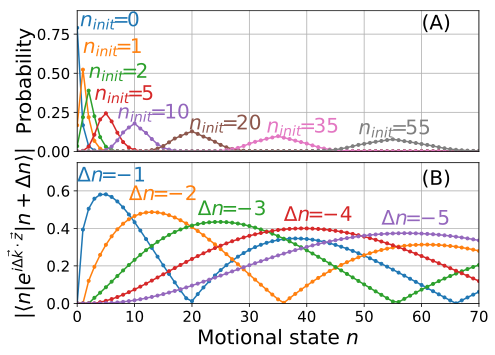
\includegraphics[width=8.5cm]{imgs/fig2_raman_op.pdf}
  \caption{Optical pumping motional-state redistribution and Raman coupling for large LD parameters for the axial direction ($z$). The range plotted covers $95$\% of the initial thermal distribution.
   % The range plotted covers $95$\% of the initial thermal distribution.
    (A) Motional state distribution %averaged over photon emission pattern
    after one OP cycle
    for different initial states motion, $n_{\textrm{init}}$. Due to photon-recoil and the large LD parameter, $\eta^{OP}_z=0.6$,
    there is a high probability of $n$ changing.         (B) Matrix elements for Raman transition deviate from
    $\sqrt{n}$ scaling with multiple minima. During cooling, we utilize the fact that high motional states couple most effectively to sidebands with large $|\Delta n|$.
    \label{f-ld}}
\end{figure}

%During optical pumping, for an atom starting in motional level $n_{\textrm{init}}$, the probability of recoil to another state $n$ is determined by the squared matrix element $|\langle n_{\textrm{init}}|e^{i \Delta k z}| n\rangle|^2$ and causes motional-state redistribution as shown in Fig.~\ref{f-ld}A.  Here $\Delta k$ is the wave vector difference between absorbed and emitted photons. The LD parameters for OP are $\{\eta^{\textrm{OP}}_x,\eta^{\textrm{OP}}_y,\eta^{\textrm{OP}}_z\} = \{0.241(2), 0.206(1), 0.602(5)\}$.  As noted already, prior to RSC, the weak axial direction %, $(\eta^{\textrm{OP}}_{z,\textrm{eff}})^2>1$ is far outside of the LD regime, and the probability of recoil per OP step is large, possibly leading to runaway heating.

%Fortunately, the large LD parameters also provide opportunities to overcome OP heating.
%The LD parameter for Raman transitions is defined as $\eta^R\equiv\Delta k z_0$,
%where the wave vector is replaced by the wave vector difference $\Delta k$
%between the two beams that drive the Raman transition.
%The Raman transitions in our configuration have LD parameters of
%$\{\eta^R_x,\eta^R_y,\eta^R_z\} = \{0.341(2), 0.291(1), 0.40(1)\}$.
%To offset heating from OP initially when $n$ is large, higher-order Raman sidebands ($\Delta n <-1$)   remove several motional quanta in a single cooling pulse (see Fig.~\ref{f-ld}B).
%Because the coupling strengths of different orders do not reach minima for the same state of motion $n$,
%using multiple orders of sidebands avoids accumulations of population
%near the coupling minima.

During optical pumping, photon recoil can lead to significant heating, especially along the weakly-confined axial direction ($z$).  For an atom starting in an axial motional level $n_{\textrm{init}}$, the probability to end in another axial state $n$ after absorbing and re-emitting one photon is approximated by an angular integral of the squared matrix element $|\langle n_{\textrm{init}}|e^{i \Delta k_{OP} z}| n\rangle|^2$ \cite{ItanoWineland1979}. Here $\Delta k_{OP}$ is the wave vector difference between absorbed and emitted photons, projected onto the $z$-axis.  As shown in Fig.~\ref{f-ld}A, the probability of gaining motional energy during OP grows with $n_{\textrm{init}}$, and is an important effect for sideband-cooling outside the Lamb-Dicke regime.

Fortunately, the large LD parameters in our system also provide opportunities to overcome OP heating.
The LD parameter for Raman transitions is defined as $\eta^R\equiv\Delta k z_0$,
where $\Delta k$ is the wave vector difference
between the two beams that drive the Raman transition.  Here $z_0=\sqrt{\hbar/(2 m \omega)}$ is the ground state wavefunction spread ($m$ is the atomic mass).
The Raman transitions in our configuration have LD parameters of
$\{\eta^R_x,\eta^R_y,\eta^R_z\} = \{0.341(2), 0.291(1), 0.40(1)\}$.
To offset heating from OP initially when $n$ is large, higher-order Raman sidebands ($|\Delta n| > 1$)   remove several motional quanta in a single cooling pulse (see Fig.~\ref{f-ld}B).
Because the coupling strengths of different orders do not reach minima for the same state of motion $n$,
using multiple orders of sidebands avoids accumulations of population
near the coupling minima.

Taking the large motional-state changing heating and cooling sources
 into account,
it is not immediately clear that ground-state cooling can be achieved.
We therefore use a Monte-Carlo simulation to guide our search~\cite{Dalibard1992}.
%and to find a robust cooling sequence~\footnote{See supplemental material}.
In particular, we find that alternating the cooling pulses (Fig.~\ref{f-setup}C) between two
neighboring orders for the axial direction and $\Delta n=-2$ and $\Delta n=-1$ for the radial directions
eliminates the accumulation of population in motional states that have zero Raman coupling, which would halt the cooling process.
The simulation also indicates that setting the coupling strength of each sideband
to drive a Rabi $\pi$-pulse corresponding to the maximum matrix element motional state
(i.e. the maxima in Fig.~\ref{f-ld}B)  yields efficient cooling, initially.
The efficiency of cooling on higher-order sidebands diminishes
as the atom approaches the ground state, so the final cycles utilize only the $\Delta n=-1$ sideband while alternating between the three axes.

Guided by the simulation results,
we construct our axial cooling sequence by starting at the two highest
observed sideband orders ($\Delta n=-8$ and $\Delta n=-7$)
and decreasing the orders to the next pair after every $6$ to $15$ cycles.
This process is repeated until $\Delta n=-1$, and most of the
population is in the first few excited states. We then switch to cooling only on $\Delta n=-1$ with two different pulse lengths in order to efficiently cool atoms in the
few remaining motional states.
Radial cooling is performed similarly to axial cooling with the initial cooling of $\Delta n=-2$ and $\Delta n=-1$ and switching to $\Delta n=-1$ only after $20$ to $30$ pulses.
This sequence gives good initial cooling performance, which is then used to calibrate experimental
parameters, including the Rabi rates of the Raman beams and optical pumping rates.

There are two additional important challenges in cooling single sodium atoms.
First, the initial temperature populates high motional states,
causing the atoms to sample the anharmonicity of the trap away from the center. Anharmonicity may be defined as $A_{i,n}=(E_{i,n+1}-E_{i,n})/h - \omega_i/(2\pi)$ for each trap axis $i$, and calculated from the quartic term of the optical tweezers via perturbation theory.
In the paraxial approximation, we find $A_{i,n}=\frac{-3n\hbar}{4\pi m d_i^2}$, where $d_i$ equals the beam radius for the radial directions and $d_z\approx\pi w_{0,x}w_{0,y}/\lambda_{\textrm{trap}}$.
%We find $A_{i,n}=\frac{3n \hbar}{4 \pi m d_i^2}$  where $d_i=w_{0,x},w_{0,y}$ for the radial directions and $d_z\approx \pi w_{0,x}w_{0,y}/\lambda$ for the axial direction.
Numerically, $\{A_{x,n},A_{y,n},A_{z,n}\}=\{-1.1, -2.0, -0.16\}n$~kHz. For mixed states, this broadens high-order sidebands due to the $n$-dependence of the transitions.
In order to mitigate this, we drive the sidebands with a large Rabi frequency
and short pulses to Fourier broaden the spectrum. %, and use Blackman pulse envelopes to avoid unwanted coupling to the carrier and heating sidebands~\cite{Kasevich1992}.
However, anharmonicity may still shift high-$n$ states out of resonance and prevent effective cooling.
%Anharmonicity may be defined as $A_{i,n}=(E_{i,n+1}-E_{i,n})/h - \omega_i/(2\pi)$ for each trap axis $i$, and calculated from the quartic term of the optical tweezers via perturbation theory.  We find $A_{i,n}=\frac{3n \hbar}{2 m d_i^2}$  where $d_i=w_0$ for the radial directions and $d_z=\pi w_0^2/\lambda$  Numerically, $\{A_{x,n},A_{y,n},A_{z,n}\}=\{1.3, 1.2, 0.2\}n$~kHz.  Anharmonicity broadens the high-order axial transitions and may shift high-$n$ states out of resonance to prevent effective cooling.

%The anharmonicity in the radial directions is calculated to be 1kHz/n, meaning that a Rabi frequency of at least $15$ kHz is needed to couple to $99$\% population up to $n=15$.


\begin{figure*}
  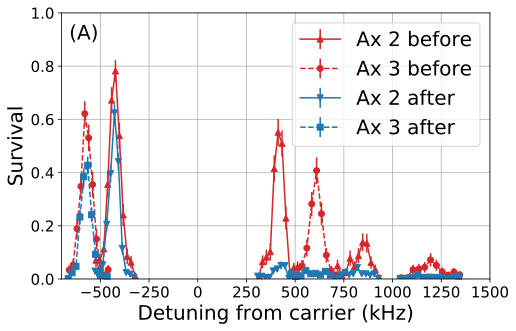
\includegraphics[height=4.2cm]{imgs/spectrum_r.pdf}
  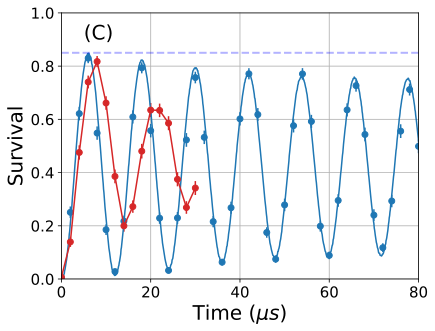
\includegraphics[height=4.2cm]{imgs/rabi_flop_r3_0.pdf}
  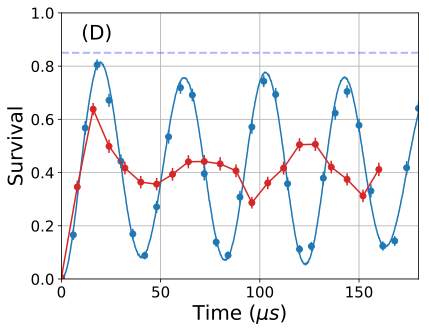
\includegraphics[height=4.2cm]{imgs/rabi_flop_r3_p1.pdf}
  \caption{(A) Left to right: Radial Raman sideband spectrum of $\Delta n_y=1,\,\Delta n_x=1,\,\Delta n_x=-1,\,\Delta n_y=-1,\,\Delta n_x=-2,\,\Delta n_y=-2$  before and after Raman sideband cooling.
    (B,C) Rabi flopping on axis $y$ (B) carrier and (C) $\Delta n_y=1$  sideband
    before (red circle) and after (blue square) RSC.
    Solid lines in (B) and (C) are
    fits to a Rabi-flopping that includes a thermal distribution of motional states~\cite{Meekhof1996}  as well as off-resonant scattering from the Raman beams.  The curves reach a maximum contrast of 85\% (horizontal dashed line) because 5\% of atoms are lost from one imaging step to the next, and 10\% of atoms are additionally lost during Raman cooling.
    The blue lines correspond to a 1D ground state probability of $93$\% after cooling (not including loss) and
    the red lines correspond to a thermal distribution of $70$ $\mu$K before RSC.
    %The horizontal dashed line shows the overall survival after cooling and imaging.
    \label{f-radial}}
\end{figure*}
\begin{figure*}
  \includegraphics[height=4.2cm]{imgs/spectrum_a1.pdf}
  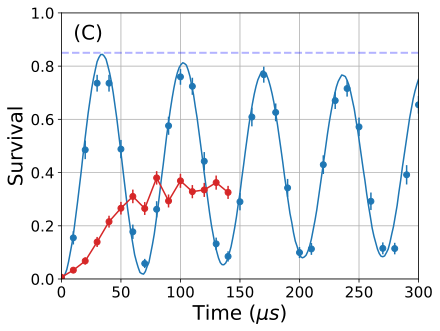
\includegraphics[height=4.2cm]{imgs/rabi_flop_a1_0.pdf}
  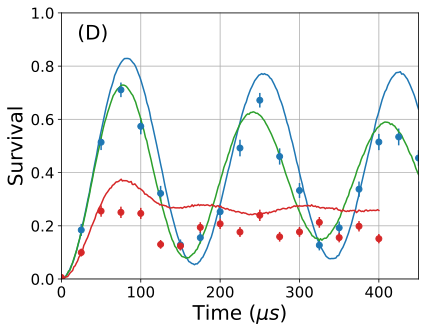
\includegraphics[height=4.2cm]{imgs/rabi_flop_a1_p1.pdf}
  \caption{(A) Left to right: Axial Raman sideband spectrum from $\Delta n_z=1,0,-1,\ldots,-8$    before and after Raman sideband cooling.
    %The data for the 2nd- and higher-orders of cooling sidebands are taken with 150 $\mu$s pulse duration and the rest are taken with 125 $\mu$s pulse duration.
    (B,C) Rabi flopping on axial (B) carrier $\Delta n_z=0$  and (C) $\Delta n_z=1$ sideband
    before (red circle) and after (blue square) RSC.
    Solid blue lines in (B) and (C), similar to Fig.~\ref{f-radial}B and C, are fits to the Rabi flopping and yield a ground state probability of $92$\% after cooling (not including the 15\% population loss) and
    the red lines correspond to a thermal distribution of $70$ $\mu$K before RSC.
    %The blue lines do not take into account the effect of decoherence due to resonance fluctuation.
    %By comparing it to
    The green line in (C), includes the additional decoherence due to a fluctuation of the hyperfine splitting of magnitude 3kHz. %a $3$ kHz fluctuation of the hyperfine splitting.
    We see that the decoherence effect is strongest for the post-cooling data on
    the $\Delta n_z=1$ sideband where the Rabi frequency is the lowest.
    %The asymptotic values for the red lines are low also because of resonance fluctuation.
    %Similar to the Figure~\ref{f-radial},
    The horizontal dashed line shows the overall survival after cooling and imaging.
    \label{f-axial}}
\end{figure*}

Second, the tweezers cause a large light shift (as large as $300$ MHz)
in the excited state. %This causes position-dependent OP detuning
%and mixes the excited-state hyperfine levels,  reducing optical pumping fidelity.
We address this by strobing the trapping light at a rate of 3 MHz during the whole cooling sequence,
similar to our loading and imaging process~\cite{Hutzler2017-LightShifts},
while leaving OP on with constant intensity.
Due to the large light shift, the OP is effectively off whenever the trap light is on.
Since the atom is still addressed by optical pumping light when the trap light is off, OP remains effective.
%  However, the selection rules that make the state |2,-2> dark to OP light are only approximately true when the tweezer light is on, and turning off the OP light during this period is expected to reduce spontaneous emission.



Our final cooling results are shown in Fig.~\ref{f-radial} and \ref{f-axial}.
In total, $1000$ cooling pulses (total duration $100$ ms) are applied
along three axes with cooling beginning on the radial second order and axial eighth order.
The full RSC pulse sequence is given in~\footnote{See supplemental material}.
To characterize the single atom thermal state before and after cooling,
we perform Raman sideband thermometry~\cite{Monroe1995, Meekhof1996}.
For the more tightly confined (non-degenerate) radial directions,
we observe clear $\Delta n=1$, $\Delta n=-1$, and $\Delta n=-2$ sidebands before RSC, as is shown in Fig.~\ref{f-radial}A.
After RSC, the $\Delta n=-1$ and $\Delta n=-2$ sidebands on both radial axes are strongly reduced.
%It is important to note that the simple sideband thermometry formula, which predicts the ratio of the cooling and heating sideband heights to be $\bar n / (\bar n + 1)$~\cite{Monroe1995}, assumes that the coupling strength for different motional states is proportional to $\sqrt{n}$. However, outside of the LD regime, the coupling strength rapidly deviates from this simple scaling rule, as shown in Figure \ref{f-ld}A. Since the Raman spectroscopy is performed with relatively large Raman LD parameters $\eta^R$, we cannot use this formula to measure $\bar n$.
The formula that equates the ratio of $\Delta n=-1$ and $\Delta n=1$ sideband heights to $\bar{n}/(\bar{n}+1)$ ($\bar{n}$ is the mean motional quantum number of the assumed thermal state) was derived in the LD regime~\cite{Monroe1995}. However, it is also valid outside the LD regime.  The resulting $\bar{n}_x=0.09(3)$ and $\bar{n}_y=0.05(2)$ correspond to ground-state fractions of 92(2)\% and 95(2)\%,  in agreement with fitted values of 89(2)\% and 92(2)\% from the Rabi flopping curves~ \cite{Meekhof1996} in Fig.~\ref{f-radial}B and \ref{f-radial}C.
%Instead, given the absence of the second order cooling sideband, we assume that the atoms are cold enough to have stronger coupling to the first order cooling sideband than the second order, i.e. below where the matrix element for the two orders cross, in which case the lower bound of the ground state population can be computed from the heights of the sidebands by assuming all of the excitations are in the $n=1$ state. In doing this, we found a ground state population of $90(2)$\% and $94(3)$\% along the two radial directions. We also use measurements of Rabi flopping on the carrier (Fig. \ref{f-radial}B) and first-order heating(Fig. \ref{f-radial}C) sidebands to verify our assumption about the distribution and the ground state population~\cite{Meekhof1996}. The data is fitted using the same Monte-Carlo simulation we used to simulate the cooling which yields $89(2)$\% and $92(2)$\% and show good agreement with the population extracted from the sideband thermometry.
The initial temperature of $70\,\mu$K before RSC is obtained
from similar fits. %the motional-state decohered Rabi flopping.

For the weak axial direction, cooling is challenging because the atom starts outside the LD regime.
We observe up to 8th-order Raman cooling sidebands initially,
which indicates population in highly-excited motional states.
Nevertheless, our cooling sequence works efficiently as all the $\Delta n<0$ sidebands are reduced
after RSC (Fig.~\ref{f-axial}A).
Using the ratio of first-order sideband heights, we obtain $\bar{n}_z=0.07(3)$, which corresponds to a ground state population of
93(3)\%, in agreement with a ground state population of 91(2)\% extracted from Rabi flopping
when $\Delta n=0$ (Fig.~\ref{f-axial}B).
For the $\Delta n=1$ sideband (Fig.~\ref{f-axial}C),
we observe additional decoherence that is more pronounced due to the slower Rabi frequency.
The decoherence rate is consistent with magnetic field fluctuations of $1.5$ mG measured independently in the lab, which would produce a Zeeman shift of $\sim 3$ kHz.

Combining the axial and radial cooling results,
 a single Na atom is in the 3D ground state with a probability of 81(4)\% after RSC.
 We note that there is an additional 5\% population loss from imaging and 10\% loss
from high-lying initial motional states that are not efficiently cooled by RSC,
but instead heated out of the trap by off-resonant scattering from the Raman beams.
The cooling efficiency is limited by spontaneous scattering rate (0.5-1 kHz) from the Raman beams, as well as spectral broadening from magnetic field fluctuations and trap anharmonicity.


We measure a heating rate that corresponds to decreasing 3D ground state population at a rate of $\sim0.9$\%/ms.
The rate is consistent with off-resonant scattering of the trapping light~\cite{Grimm2000}, and is predominantly in the axial direction where the trapping beam propagates.
%The ground state probability achieved is currently limited by off-resonant scattering from the Raman beams, which are measured to be between $3$ to $15$ kHz for the detuning and power we use, and the resonance shift caused by magnetic field fluctuations.


%Taking into account the population loss, from each successful single atom loading event, we can currently prepared a single \textit{Na} atom in the 3D ground-state with an overall $66(3)$\% fidelity.
We expect to reduce atom losses and enhance the ground state probability after RSC
by increasing the detuning of the Raman beams,
addressing a wider range of axial trap anharmonicity, % by frequency sweeps,
implementing better control of the magnetic field, and optimizing imaging.
Another improvement could be to implement grey molasses cooling to achieve
a lower starting temperature before RSC~\cite{Colzi2016}.

%\fxnote{The distinction between 77 and 66 percent is confusing, we should discuss it}

We have shown that despite the difficulty in achieving a low optical cooling temperature
of low mass sodium atoms,  three dimensional cooling
with significant ground state population can be achieved by using high-order Raman sidebands
in an optimized cooling sequence.
These techniques are well-suited for a large variety of systems
and open up a route to ground state cooling for other species, including molecules and exotic atoms.

We thank J. D. Hood for discussions.
This work is supported by the Arnold and Mabel Beckman Foundation, the AFOSR Young Investigator Program, the NSF through the CUA,
and the Alfred P. Sloan Foundation.

% Lamb-Dicke parameter square explain
% why not just molecules instead of polar molecules
% use entropy to describe the effect of large \eta_{eff}
% 1 sentence to explain why anisotropy?
% Mention after cooling is non-thermal?

\bibliography{paper}
\end{document}
